% Modern editorial, markup and figure/layout contributions: CC-BY-SA-4.0.
% Historical text and illustrations: Leonhard Euler (1744), public domain.
% Component scope and upstream attribution: see RIGHTS.md.
% Manual vector redraw from E65 Tabula I, Fig. 7.
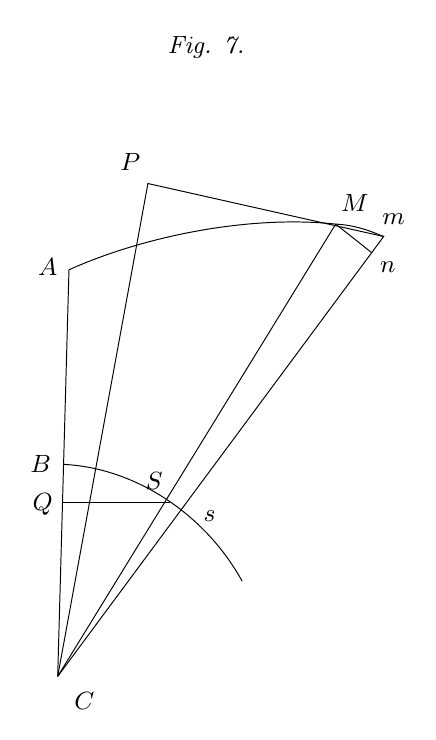
\begin{tikzpicture}[x=1cm,y=1cm,line width=.35pt,font=\small]
\draw (0.7664,0.3008)--(0.9096,5.4647);
\draw (0.7664,0.3008)--(1.9123,6.5605)--(4.9061,5.8873)--(0.7664,0.3008);
\draw (0.7664,0.3008)--(4.2973,6.0449);
\draw (4.2973,6.0449)--(4.7485,5.6868);
\draw (0.8308,2.5139)--(2.1916,2.5139);
\draw (0.9096,5.4647) .. controls (1.8980,5.9088) and (3.2373,6.1595) .. (4.2973,6.0449) .. controls (4.5623,6.0305) and (4.7485,5.9518) .. (4.9061,5.8873);
\draw (0.8380,2.9938) .. controls (1.7547,2.9508) and (2.6428,2.3564) .. (3.1084,1.5112);
\node[anchor=east,inner sep=1pt] at (0.8022,5.5005) {$A$};
\node[anchor=east,inner sep=1pt] at (0.7234,3.0009) {$B$};
\node[anchor=east,inner sep=1pt] at (0.7449,2.4853) {$Q$};
\node[anchor=north west,inner sep=1pt] at (0.9382,0.1432) {$C$};
\node[anchor=south east,inner sep=1pt] at (1.8550,6.6823) {$P$};
\node[anchor=south west,inner sep=1pt] at (4.3259,6.1595) {$M$};
\node[anchor=south west,inner sep=1pt] at (4.8488,6.0019) {$m$};
\node[anchor=north west,inner sep=1pt] at (4.8201,5.6080) {$n$};
\node[anchor=south east,inner sep=1pt] at (2.1415,2.6285) {$S$};
\node[anchor=west,inner sep=1pt] at (2.5784,2.3349) {$s$};
\node[anchor=south] at (2.6500,8.0216) {\textit{Fig. 7.}};
\end{tikzpicture}
